\chapter{State of the Art}

\section*{Introduction}
\phantomsection
\addcontentsline{toc}{section}{Introduction}
The state of the art constitutes the preliminary phase of our project where we study the existing landscape, identify shortcomings in current solutions, and define our project's requirements. In this chapter, we begin by presenting the project context, study existing solutions, propose our solution, specify functional and non-functional requirements, and define our working methodology.
\section{Context and Problem Statement}
Social media management has become a critical business function for content creators, influencers, and enterprises. Managing content across multiple platforms---YouTube, TikTok, Instagram, Facebook, and Snapchat---requires significant effort in content creation, scheduling, and performance monitoring.

BViral Control Center was conceived as a comprehensive solution to centralize all social media management tasks into a single, powerful dashboard. The project is developed as a full-stack web application with an integrated AI video enhancement pipeline, targeting content creators who need to manage their multi-platform presence efficiently.
% ── FIGURE: Place your project logo here ──
% \begin{figure}[H]
%     \centering
%     
\includegraphics[width=0.3\textwidth]{figures/bviral_logo.png}
%     \caption{BViral Control Center Logo}
%     \label{fig:bviral-logo}
% \end{figure}
\subsection{Study of Existing Solutions}

\subsubsection{Analysis of Existing Solutions}

Before developing our solution, we conducted a thorough study of the main existing social media management platforms:

\textbf{Hootsuite:} is one of the most popular social media management platforms. It allows users to schedule posts, manage multiple accounts, and track analytics from a single dashboard. Hootsuite supports major platforms including Facebook, Instagram, Twitter, LinkedIn, and YouTube.

% ── FIGURE: Screenshot of Hootsuite ──
% \begin{figure}[H]
%     \centering
%     \includegraphics[width=0.8\textwidth]{figures/hootsuite.png}
%     \caption{Existing solution: Hootsuite Dashboard}
%     \label{fig:hootsuite}
% \end{figure}

% ── FIGURE: Screenshot of Hootsuite ──
% \begin{figure}[H]
%     \centering
%     \includegraphics[width=0.8\textwidth]{figures/hootsuite.png}
%     \caption{Existing solution: Hootsuite Dashboard}
%     \label{fig:hootsuite}
% \end{figure}
% ── FIGURE: Screenshot of Buffer ──
% \begin{figure}[H]
%     \centering
%     \includegraphics[width=0.8\textwidth]{figures/buffer.png}
%     \caption{Existing solution: Buffer}
%     \label{fig:buffer}
% \end{figure}
\textbf{Topaz Video AI:} is a desktop application specializing in AI-powered video enhancement. It uses deep learning models to upscale, denoise, and sharpen videos. However, it is a standalone desktop tool with no social media integration.
\subsubsection{Critique of Existing Solutions}

The existing solutions present several limitations:

\textbf{Hootsuite:} offers comprehensive scheduling and analytics but lacks any AI-powered video enhancement capability. Its pricing model is expensive for individual creators, and it does not support TikTok natively with full features. The video editing capabilities are minimal.
\textbf{Buffer:} provides a simple and clean interface but offers limited analytics compared to competitors. It lacks video enhancement features entirely and has restricted support for newer platforms like TikTok and Snapchat.

\textbf{Topaz Video AI:} delivers excellent AI video enhancement with models like Real-ESRGAN and GFPGAN, but it operates only as a standalone desktop application. It has no scheduling, analytics, or social media management features.


\begin{table}[H]
\centering
\caption{Comparison of existing solutions}
\label{tab:comparison}
\begin{tabularx}{\textwidth}{|l|X|X|X|X|}
\hline
\textbf{Feature} & \textbf{Hootsuite} & \textbf{Buffer} & \textbf{Topaz AI} & \textbf{BViral (Ours)} \\
\hline
Multi-platform scheduling & \checkmark & \checkmark & $\times$ & \checkmark \\
\hline
Analytics dashboard & \checkmark & Limited & $\times$ & \checkmark \\
\hline
AI video enhancement & $\times$ & $\times$ & \checkmark & \checkmark \\
\hline
OAuth account connection & \checkmark & \checkmark & $\times$ & \checkmark \\
\hline
Integrated video editor & $\times$ & $\times$ & \checkmark & \checkmark \\
\hline
Alert management & Limited & $\times$ & $\times$ & \checkmark \\
\hline
Open-source / Self-hosted & $\times$ & $\times$ & $\times$ & \checkmark \\
\hline
Free for individuals & $\times$ & Limited & $\times$ & \checkmark \\
\hline
\end{tabularx}
\end{table}

\subsection{Suggested Solution}

We propose \textbf{BViral Control Center}, a web-based platform that combines social media management with AI-powered video enhancement in a single, unified interface. Our solution addresses the gaps identified in existing tools by providing:

\begin{itemize}
    \item A centralized dashboard for managing posts across YouTube, TikTok, Instagram/Facebook, and Snapchat.
    \item An integrated scheduling system with a visual calendar interface backed by Redis queues for reliable post publishing.
    \item OAuth-based account connection for YouTube, TikTok, and Meta (Facebook/Instagram) with PKCE security.
    \item A comprehensive analytics module with performance metrics, engagement tracking, and revenue monitoring.
    \item An AI-powered video enhancement pipeline using Real-ESRGAN for super-resolution and GFPGAN for face restoration.
    \item An integrated browser-based video editor (BVIRAL Video Editor) for timeline editing, media import, and export.
    \item An alert management system for monitoring errors, copyright issues, and success notifications.
\end{itemize}




\section{Theoretical Background and AI Concepts}
This section introduces the fundamental theoretical concepts of AI and presents the core algorithms utilized in this project, fulfilling the prerequisite knowledge required for our pipeline.

\subsection{Basic Concepts of Artificial Intelligence}
Artificial Intelligence in our system relies on two primary paradigms of Machine Learning:
\begin{itemize}
    \item \textbf{Supervised Learning:} A paradigm where the model learns from a labeled dataset. The algorithm is provided with input features and the known correct output (the target). Its goal is to map the function connecting inputs to outputs. In our project, predicting video views is a supervised regression task.
    \item \textbf{Unsupervised Learning:} A paradigm where the model identifies hidden patterns in unlabeled data without predefined target variables. We utilize this paradigm primarily for dimensionality reduction, compressing complex data while retaining its core mathematical structure.
\end{itemize}

\subsection{Presentation of Domain-Specific Algorithms}
Our system integrates several state-of-the-art algorithms across Machine Learning, Computer Vision, and Natural Language Processing:

\begin{itemize}
    \item \textbf{XGBoost (eXtreme Gradient Boosting):} An advanced implementation of gradient boosted decision trees designed for speed and performance. It is mathematically optimized for structured, tabular data. We utilize XGBoost as our primary supervised regression algorithm to predict the algorithmic reach (\texttt{log\_views}) of a video.
    \item \textbf{PCA (Principal Component Analysis):} An unsupervised linear transformation technique used for dimensionality reduction. It projects high-dimensional data (e.g., 512-dimensional visual embeddings) into a lower-dimensional subspace while preserving the maximum possible variance, preventing the "Curse of Dimensionality" in our predictive model.
    \item \textbf{GANs (Generative Adversarial Networks):} Deep learning architectures composed of a Generator and a Discriminator that compete against each other to create highly realistic synthetic data. We utilize specific GAN variations (\textbf{Real-ESRGAN} and \textbf{GFPGAN}) in our video enhancement pipeline to hallucinate missing pixels for super-resolution and facial restoration.
    \item \textbf{Transformers and Foundation Models:} Attention-based neural network architectures that excel at processing sequential data. Our system heavily relies on pre-trained foundation models, including \textbf{OpenAI Whisper} for speech-to-text, \textbf{CLIP} for zero-shot image classification and visual embeddings, and \textbf{Llama 3} for abstract semantic reasoning.
\end{itemize}

\section{Actors and Needs Identification}
Before establishing the exact technical capabilities of the \textit{BViral Control Center}, it is essential to align the system design with its end-users and operational constraints. The platform primarily serves two main actors: the \textbf{Content Creator/Social Media Manager}, who requires a streamlined, automated, and intelligent environment to optimize their cross-platform workflow, and the \textbf{System Administrator}, who ensures platform stability, handles infrastructure configuration, and monitors global execution queues. 

To satisfy the specific expectations of these actors and ensure seamless operations, the system must adhere to a strict set of capabilities. These are formally divided into explicit behavioral features, which dictate the daily operational tools available to the user, and qualitative constraints, which govern the architectural robustness, security, and scalability of the platform.
\subsection{Functional Requirements}
Our solution must satisfy the following functional requirements:

\begin{longtable}{|p{4cm}|p{10cm}|}
\caption{Functional requirements of BViral Control Center}
\label{tab:functional-requirements} \\
\hline
\textbf{Module} & \textbf{Functional Requirements} \\
\hline
\endfirsthead

\hline
\textbf{Module} & \textbf{Functional Requirements} \\
\hline
\endhead

Account Management &
\begin{itemize}
    \item Connect and disconnect YouTube accounts via Google OAuth 2.0.
    \item Connect and disconnect TikTok accounts via TikTok OAuth with PKCE.
    \item Connect and disconnect Meta (Facebook/Instagram) accounts via Facebook Login.
    \item View all connected accounts with platform, name, and connection status.
\end{itemize} \\
\hline

Post Scheduling &
\begin{itemize}
    \item Create new scheduled posts with video, caption, and target platform.
    \item View scheduled, posted, and failed posts in a calendar interface.
    \item Cancel or reschedule pending posts.
    \item Publish posts automatically at their scheduled time through a background worker.
\end{itemize} \\
\hline

Analytics &
\begin{itemize}
    \item View aggregated analytics: views, likes, comments, shares, and revenue.
    \item Filter analytics by platform and time period.
    \item Visualize performance trends with interactive charts.
\end{itemize} \\
\hline

AI Video Studio &
\begin{itemize}
    \item Enhance video quality using Real-ESRGAN super-resolution (2x/4x).
    \item Apply GFPGAN face restoration on detected faces.
    \item Apply classical filters: denoise, deblur, and color correction.
    \item Preview before/after comparisons and quality metrics (PSNR, SSIM, LPIPS).
    \item Access the integrated BVIRAL Video Editor for timeline editing.
\end{itemize} \\
\hline

Alerts &
\begin{itemize}
    \item Receive alerts for posting errors, copyright issues, and success notifications.
    \item Mark alerts as resolved or unresolved.
    \item Filter alerts by type, platform, and status.
\end{itemize} \\
\hline
\end{longtable}

\subsection{Non-functional Requirements}
The system must also satisfy the following quality and technical constraints:

\begin{longtable}{|p{4cm}|p{10cm}|}
\caption{Non-functional requirements of BViral Control Center}
\label{tab:non-functional-requirements} \\
\hline
\textbf{Category} & \textbf{Requirement} \\
\hline
\endfirsthead

\hline
\textbf{Category} & \textbf{Requirement} \\
\hline
\endhead

Security & OAuth 2.0 with PKCE for TikTok; AES-256 encryption for stored access tokens; Supabase Row Level Security (RLS) policies on all database tables; JWT-based authentication. \\
\hline

Performance & Redis/BullMQ queues for reliable asynchronous post publishing; parallel CPU processing for AI video enhancement when GPU is unavailable. \\
\hline

Scalability & pnpm monorepo workspace architecture separating frontend, backend, and shared libraries; modular service layer in the API server. \\
\hline

Maintainability & TypeScript across the entire stack; Drizzle ORM with type-safe database schema; OpenAPI specification with generated Zod validation schemas. \\
\hline

Ergonomics & Modern, responsive UI built with React, Tailwind CSS, and Framer Motion animations; dark-mode dashboard design. \\
\hline

Interoperability & RESTful API with versioned routes (\texttt{/api/v1/}); standard OAuth flows compatible with all major platforms. \\
\hline
\end{longtable}

\section{Working Methodology}

Because BViral Control Center is a hybrid project combining a full-stack SaaS application with advanced Machine Learning pipelines, we adopted a dual-methodology approach: \textbf{V-Model methodology} for software engineering, and \textbf{CRISP-DM} for the artificial intelligence lifecycle.

\subsection{Software Methodology: V-Model}

To ensure a structured, reliable, and well-documented development process for the BViral Control Center platform, we adopted the \textbf{V-Model methodology} as the primary software engineering approach.

The BViral Control Center is a complex full-stack web application that integrates multiple interconnected components, including social media APIs (YouTube, TikTok, Meta), a scheduling engine based on background workers and Redis queues, an analytics dashboard, authentication and security mechanisms (OAuth 2.0, JWT, RLS), as well as an AI-powered video enhancement pipeline. Given this level of complexity and the need for reliability, a rigorous methodology was required.

The V-Model is an extension of the classical waterfall model where each development phase is associated with a corresponding testing phase. It ensures strong validation and verification throughout the entire lifecycle.

The left side of the V (design phase) includes:
\begin{itemize}
    \item Requirements analysis of the platform
    \item Functional and non-functional specifications
    \item System architecture design (frontend, backend, AI modules, database)
    \item API design and integration planning
    \item Security design (OAuth 2.0, JWT, encryption, RLS)
\end{itemize}

The right side of the V (validation phase) includes:
\begin{itemize}
    \item Unit testing of individual modules (authentication, scheduling, analytics)
    \item Integration testing between system components
    \item System testing of the full platform
    \item Validation of AI outputs using metrics (PSNR, SSIM, LPIPS)
    \item Security and performance testing
\end{itemize}

\textbf{Justification for using the V-Model}

The V-Model was chosen for several reasons. First, the project requires a high level of reliability, especially for critical features such as scheduling and authentication. The model ensures that each requirement is validated through a corresponding test.

Second, the system is composed of multiple interconnected modules (AI, backend services, APIs, frontend dashboard). The V-Model provides clear traceability between requirements, design, and testing, reducing integration risks.

Third, test cases are defined early in the development process, which allows early detection of errors, especially in API integrations and security flows.

Finally, the V-Model provides strong documentation and structure, which is essential for both maintainability and academic presentation.

\textbf{Advantages of the V-Model in this project}
\begin{itemize}
    \item High reliability through systematic verification and validation
    \item Clear traceability between requirements and test cases
    \item Early detection of design and implementation errors
    \item Better organization of complex multi-module development
    \item Strong documentation and maintainability
    \item Reduced integration risks between AI and software components
\end{itemize}

In conclusion, the V-Model is well suited to the BViral Control Center project due to its structured approach and strong emphasis on quality assurance.

\begin{figure}[H]
    \centering
    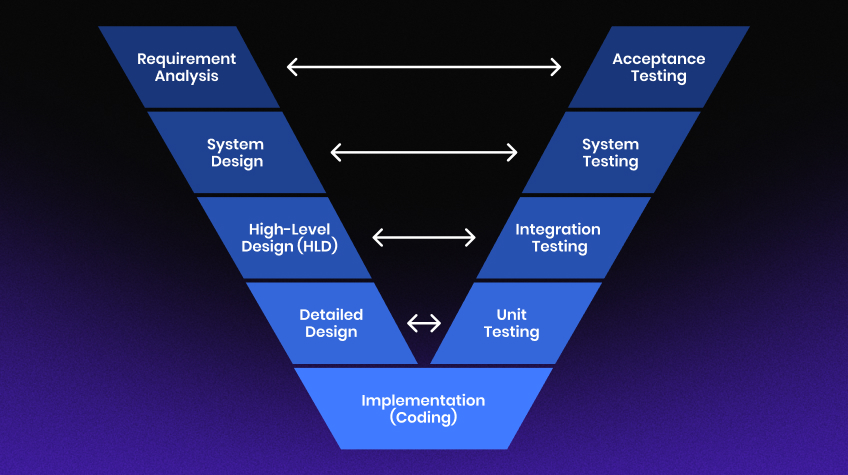
\includegraphics[width=0.85\textwidth]{logos/vmodel.jpg}
    \caption{V-Model methodology}
    \label{fig:v-model-methodology}
\end{figure}
\subsection{Software :Gantt Diagram}

% ── FIGURE: Gantt diagram (use StarUML or draw manually) ──
 \begin{figure}[H]
     \centering
     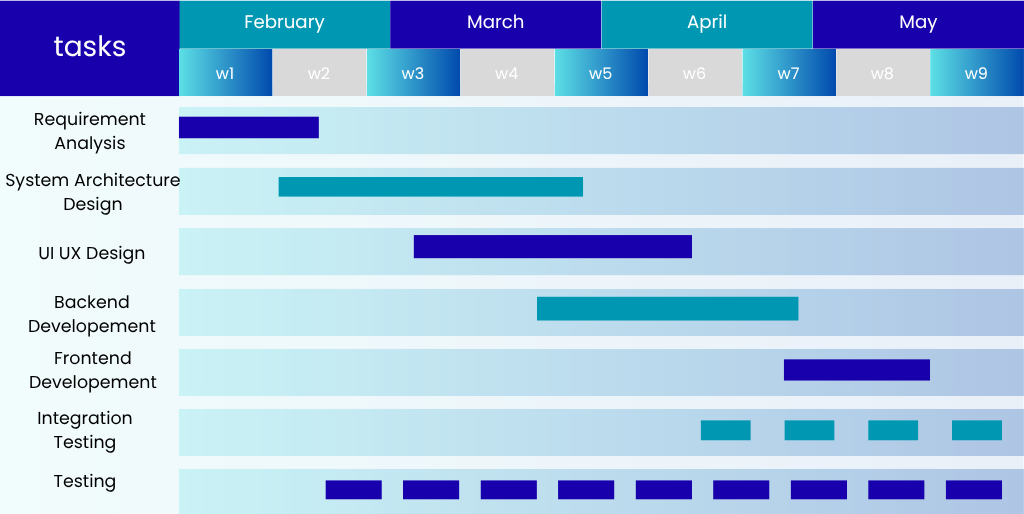
\includegraphics[width=\textwidth]{diagram/gant.png}
     \caption{Gantt diagram of the project}
     \label{fig:gantt}
 \end{figure}
\subsection{Artificial Intelligence: CRISP-DM Methodology } 
For the data science and AI modeling components, we strictly adhered to the \textbf{CRISP-DM} (Cross-Industry Standard Process for Data Mining) methodology. This industry-standard framework ensured our AI models remained focused on solving the core business problem. The six phases were implemented as follows:

\begin{enumerate}
    \item \textbf{Business Understanding:} We identified that content creators lack predictive insights before publishing. The objective was defined as building a Pre-Posting Predictive Agent to act as an algorithmic coach.
    \item \textbf{Data Understanding:} We collected over 1,100 short-form videos. Through Exploratory Data Analysis (EDA), we discovered the highly skewed power-law distribution of video views, which informed our mathematical approach.
    \item \textbf{Data Preparation:} We merged cross-platform metadata, sliced \texttt{.mp4} files into audio/visual components via FFmpeg, and applied Principal Component Analysis (PCA) to compress high-dimensional foundation model embeddings.
    \item \textbf{Modeling:} We trained and tuned multiple algorithms: XGBoost for tabular regression, \texttt{faster-whisper} for speech-to-text, and Real-ESRGAN/GFPGAN for Computer Vision upscaling.
    \item \textbf{Evaluation:} Models were rigorously tested using standard metrics (RMSE, $R^2$, PSNR). Crucially, evaluation led to the strategic decision to discard a noisy "Post-Posting" engagement model in favor of the highly accurate Pre-Posting agent.
    \item \textbf{Deployment:} The validated machine learning models were serialized and integrated into the Node.js Fastify backend, making them accessible to the end-user via the React interface.
\end{enumerate}
\subsection{Artificial Intelligence: Gantt Diagram}

% ── FIGURE: Gantt diagram (use StarUML or draw manually) ──
 \begin{figure}[H]
     \centering
     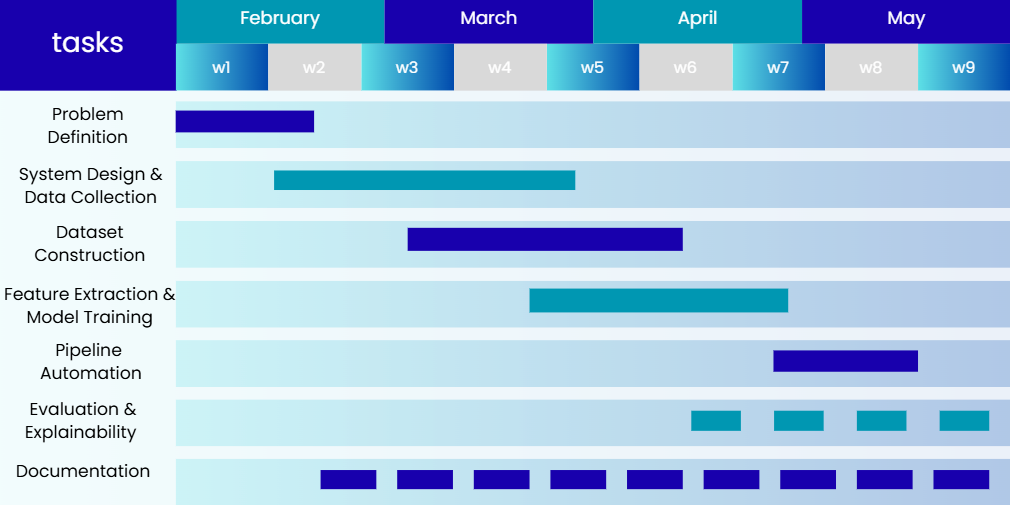
\includegraphics[width=\textwidth]{images/ganttAI.png}
     \caption{Gantt diagram of the AI part }
     \label{fig:gantt_AI}
 \end{figure}


\section*{Conclusion}
\phantomsection
\addcontentsline{toc}{section}{Conclusion}

In this chapter, we presented the general context of the \textbf{BViral Control Center} project and highlighted the growing challenges faced by content creators in managing and optimizing their presence across multiple social media platforms. Through the study and critical analysis of existing solutions such as Hootsuite, Buffer, and Topaz Video AI, we identified several limitations, particularly the lack of integration between social media management and AI-powered video enhancement.

To address these shortcomings, we proposed a unified and intelligent platform that combines scheduling, analytics, account management, AI video enhancement, and integrated video editing within a single ecosystem. We also introduced the theoretical foundations and state-of-the-art technologies adopted in our solution, including Machine Learning, Explainable AI, Computer Vision, and modern multimodal models.

Furthermore, we defined the functional and non-functional requirements of the system and presented the Agile iterative methodology selected for the project development. This methodology ensures flexibility, modularity, and continuous improvement throughout the implementation process.

The next chapter will focus on the system analysis and design phase, where we will present the global architecture, modeling diagrams, database design, and the technical structure of the proposed solution.